\documentclass[a4paper,11pt]{article}
\usepackage[T1]{fontenc}
\usepackage{lmodern}
\usepackage[margin=25mm]{geometry}
\usepackage{amsmath,amssymb,amsthm}
\usepackage{booktabs}
\usepackage{microtype}
\usepackage{array}
\usepackage{url}
\ifdefined\kanjiskip
  \PassOptionsToPackage{dvipdfmx}{graphicx}
  \PassOptionsToPackage{dvipdfmx}{xcolor}
\fi
\usepackage{tikz}
\usetikzlibrary{shapes.geometric,shapes.misc,decorations.pathreplacing,positioning,fit}

\newtheorem{theorem}{Theorem}
\newtheorem{proposition}[theorem]{Proposition}
\newtheorem{lemma}[theorem]{Lemma}
\newtheorem{corollary}[theorem]{Corollary}
\theoremstyle{definition}
\newtheorem{definition}[theorem]{Definition}
\theoremstyle{remark}
\newtheorem{remark}[theorem]{Remark}

\newcommand{\Code}{\mathit{Code}}
\newcommand{\pos}{\mathit{pos}}
\newcommand{\rmL}{\mathrm{L}}
\newcommand{\rmR}{\mathrm{R}}
\newcommand{\rmZ}{\mathrm{Z}}

\title{Smaller Universal Reversible Turing Machines\\
 and the Nonexistence of Two-State Ones}
\author{Tetsuo Yokoyama\\Nanzan University}
\date{October 2026}

\begin{document}
\maketitle

\begin{abstract}
A reversible Turing machine (RTM) is a Turing machine in which every instantaneous description has at most one predecessor.
Morita's book (2017) lists nine universal RTMs (URTMs); we write URTM$(m,n)$ for one with $m$ states and $n$ symbols.
We construct seven URTMs that are not dominated by any of these nine: URTM$(3,600)$, URTM$(4,42)$, URTM$(5,39)$, URTM$(6,30)$, URTM$(7,28)$, URTM$(8,21)$, and URTM$(85,2)$.
Together with six of Morita's machines, they give 13 non-dominated points.
The new machines come from improved versions of Morita's conversions to three states, to four states, and to two symbols.
We use a numbering of states by the direction of entry, counting in the reverse direction, a block decomposition of state numbers that trades states for symbols, and the merging of symbols that are never read or written in the same context.
For example, the improved conversion to three states uses $O(mn^2)$ symbols instead of $O(m^2n^3)$, and it turns URTM$(32,3)$ into URTM$(3,600)$ instead of URTM$(3,36654)$.
On the negative side, we show that the halting problem of RTMs with at most two states is decidable for finite instantaneous descriptions, by a single procedure that also takes the machine as input.
Consequently, there is no URTM with at most two states, which answers a question left open by Morita.
We also show that no three-state, two-symbol RTM is universal.
All these results are formalized in Lean~4 with Mathlib.
Universality is formalized after Morita's definition, with computable encoding and decoding functions, which we give explicitly for all 13 points.
\end{abstract}

\section{Introduction}

Reversible computing concerns computations in which each step uniquely determines its predecessor.
Bennett showed that irreversible computations can be simulated reversibly without loss of computational power~\cite{Bennett73}.
A reversible Turing machine (RTM) is one of the basic models of reversible computing, and a universal RTM is called a URTM.
As for ordinary universal Turing machines (UTMs)~\cite{Rogozhin96,KudlekRogozhin02,NearyWoods09,WoodsNeary09}, a natural question is how small a URTM can be.
We measure the size by the numbers of states and symbols, and write URTM$(m,n)$ for a URTM with $m$ states and $n$ symbols.

Morita's book~\cite{Morita17} lists nine URTMs.
Six of them, URTM$(10,8)$, $(13,7)$, $(15,6)$, $(17,5)$, $(24,4)$, and $(32,3)$, simulate cyclic tag systems with halting condition directly; URTM$(17,5)$ is due to Morita and Yamaguchi.
The other three, URTM$(4,168)$, $(138,2)$, and $(3,36654)$, are obtained from them by general conversions that reduce the number of states or of symbols.
The book remarks that these three leave room for reduction, and it states that the existence of a two-state URTM is open.
In a later survey, after recalling that two-state TMs are universal in the irreversible case, Morita writes that ``it is unknown whether the class of two-state RTMs is universal''~\cite{Morita23}.

\paragraph{Contributions.}
\begin{itemize}
\item \emph{New upper bounds} (Section~\ref{sec:constr}).
We give seven URTMs, $(3,600)$, $(4,42)$, $(5,39)$, $(6,30)$, $(7,28)$, $(8,21)$, and $(85,2)$, none of which is dominated by Morita's nine points (Figure~\ref{fig:compare}).
The three-state machine improves the conversion of Morita's Theorem~5.6, the machines with four to eight states come from a block decomposition of the conversion of Theorem~5.5 followed by symbol merging, and the two-symbol machine optimizes the conversion of Theorem~5.4.
No conversion in the book yields five to nine states; the block decomposition gives a whole family of state-symbol trade-offs.
\item \emph{Universality in the sense of Morita's definition} (Section~\ref{sec:univ}).
Morita's Definition~7.1 asks for total recursive encoding and decoding functions, but the book does not give them for its URTMs.
We give computable encodings and decodings for all 13 non-dominated points and prove universality in this sense.
\item \emph{Nonexistence for two states} (Section~\ref{sec:twostate}).
The halting problem of RTMs with at most two states is decidable for finite instantaneous descriptions, uniformly in the machine.
Hence no URTM with at most two states exists, for any number of symbols.
The key fact is that, in a two-state RTM, the state equals the direction of the last move, so a half-line of the tape can tell the rest of the tape only that the head has come back.
\item \emph{Nonexistence for three states and two symbols} (Section~\ref{sec:threetwo}).
No three-state, two-symbol RTM is universal.
\item \emph{Formalization} (Section~\ref{sec:formal}).
All theorems above are formalized and proved in Lean~4~\cite{Lean4} with Mathlib~\cite{Mathlib20}, using only the standard axioms.
The formalized machine model reproduces the halting step counts of the published test runs of all nine of Morita's machines.
\end{itemize}
For each number of states, the constructions give an upper bound on the minimum number of symbols of a URTM. We do not claim that any of the new points is minimal.

\paragraph{Related work.}
Small UTMs have been studied for a long time; Woods and Neary survey the results~\cite{WoodsNeary09}.
The non-dominated small UTMs listed in Morita's book include UTM$(2,18)$ and UTM$(4,6)$ of Rogozhin~\cite{Rogozhin96}, UTM$(3,9)$ of Kudlek and Rogozhin~\cite{KudlekRogozhin02}, and UTM$(5,5)$, $(6,4)$, $(9,3)$, and $(15,2)$ of Neary and Woods~\cite{NearyWoods09}.
These machines need not be reversible, and their conventions on halting and on stationary moves differ from those used here.
The URTMs of Morita and his coauthors are collected in~\cite[Ch.~7]{Morita17}, together with the conversions that we improve.
Turing machines and universal Turing machines have been formalized in Isabelle/HOL~\cite{XuZhangUrban13}, Matita~\cite{AspertiRicciotti15}, and Coq~\cite{ForsterKunzeWuttke20}, and Mathlib contains a universal partial recursive function~\cite{Carneiro19}.
These formalizations treat general constructions rather than small machines, and none of them is about reversible computation.
Closest to our two-state result is Dudenhefner's decision procedure, certified in Coq, for the halting problem of reversible two-counter machines with a particular instruction set; it contrasts with Morita's result that reversible two-counter machines with another instruction set are universal~\cite{Dudenhefner22}.
To our knowledge, small URTMs and their universality in the sense of Definition~7.1 have not been formalized before.

\section{Preliminaries}
\label{sec:prelim}

We follow Morita's book~\cite{Morita17} and state the definitions in the form used in the formalization.

\begin{definition}[Machines and runs]
A \emph{quintuple} $r=[p,s,t,D,q]$ consists of a source state $p$, a read symbol $s$, a written symbol $t$, a direction $D\in\{\rmL,\rmZ,\rmR\}$, and a target state $q$, where $p,s,t,q\in\mathbb{N}$.
The directions L, Z, and R move the head by $-1$, $0$, and $+1$; a quintuple with direction Z is a \emph{zero-shift}.
A Turing machine (TM) is a finite list $T$ of quintuples; only membership in $T$ matters.
An \emph{instantaneous description} (ID) is a triple $(\mathit{st},\pos,\mathit{tape})$ with $\mathit{st}\in\mathbb{N}$, $\pos\in\mathbb{Z}$, and $\mathit{tape}:\mathbb{Z}\to\mathbb{N}$; the symbol 0 is the blank.
A quintuple $r$ applies to an ID $\alpha$ if $r.p=\alpha.\mathit{st}$ and $r.s=\alpha.\mathit{tape}(\alpha.\pos)$; the result writes $r.t$ at $\alpha.\pos$, moves the head by the displacement of $r.D$, and enters $r.q$.
An ID is \emph{halting} for $T$ if no quintuple of $T$ applies to it.
We write $\mathrm{Halts}_T(\alpha)$ if $T$ reaches a halting ID from $\alpha$ in finitely many (possibly zero) steps.
\end{definition}

\begin{definition}[Determinism and reversibility]
$T$ is \emph{deterministic} if any two quintuples of $T$ with the same source state and read symbol are equal.
$T$ is \emph{reversible} if any two distinct quintuples of $T$ with the same target state have the same direction and different written symbols.
\end{definition}

This is Morita's Definition~5.4, specialized to the quintuple form.
By reversibility, all quintuples entering a state move in the same direction (the unique shift-direction property, \cite[Lemma~5.5]{Morita17}).
For an RTM $T$ we write $Q_+$ and $Q_-$ for the sets of states entered by right moves and by left moves, and $m_+=|Q_+|$, $m_-=|Q_-|$.

\begin{definition}[Size]
$\mathrm{NStates}(T)$ is the number of distinct source states of $T$, and $\mathrm{NSyms}(T)$ is the number of elements of $\{0\}\cup\{r.s,r.t\mid r\in T\}$.
A point $(m,n)$ \emph{dominates} $(m',n')$ if $m\le m'$, $n\le n'$, and $(m,n)\ne(m',n')$.
\end{definition}

Halting states, which have no outgoing quintuples, are not counted, as in Morita's book (Section~\ref{sec:counting}).

\paragraph{Codes of finite IDs.}
An ID is \emph{finite} if it has finitely many non-blank cells.
Let $\Code=\mathbb{N}\times\mathrm{List}\,\mathbb{N}\times\mathrm{List}\,\mathbb{N}$.
For $p\in\mathbb{Z}$ and $(q,l,r)\in\Code$, the ID $\mathrm{toID}(p,(q,l,r))$ has state $q$ and head position $p$, carries $r$ on the cells $p,p+1,\dots$ and $l$ on the cells $p-1,p-2,\dots$, and is blank elsewhere.
For an ID $\alpha$, $\alpha.\pos$ is its head position.
$\mathrm{IsIDOf}(T,\alpha)$ holds if $\alpha$ is finite, its state occurs in $T$, and every cell holds the blank or a symbol occurring in $T$.
The enumeration $\mathrm{tm}(i)$, $i\in\mathbb{N}$, decodes $i$ into a list of quintuples by the standard bijection between $\mathbb{N}$ and lists of tuples of natural numbers in Mathlib, and replaces a non-deterministic result by the empty list.

\begin{definition}[Universality, after {\cite[Def.~7.1]{Morita17}}]
\label{def:univ}
A table $U$ satisfies $\mathrm{IsUTMStrict}(U)$ if there are an encoding $c:\mathbb{N}\times\Code\to\Code$ and a decoding $d:\Code\to\mathrm{Option}\,\Code$, both computable, such that for all $i\in\mathbb{N}$ and all $a\in\Code$ with $\mathrm{IsIDOf}(\mathrm{tm}(i),\mathrm{toID}(0,a))$:
\begin{enumerate}
\item $\mathrm{IsIDOf}(U,\mathrm{toID}(0,c(i,a)))$;
\item if $\mathrm{tm}(i)$ reaches a halting ID $\beta$ from $\mathrm{toID}(0,a)$, then $U$ reaches a halting ID $\gamma$ from $\mathrm{toID}(0,c(i,a))$, $\gamma$ has a code (some $g$ with $\mathrm{toID}(\gamma.\pos,g)=\gamma$), and every such code $g$ satisfies $d(g)=\mathrm{some}(b)$ for some $b$ with $\mathrm{toID}(\beta.\pos,b)=\beta$;
\item if $\mathrm{tm}(i)$ does not halt from $\mathrm{toID}(0,a)$, then $U$ does not halt from $\mathrm{toID}(0,c(i,a))$.
\end{enumerate}
The weaker predicate $\mathrm{IsUTM}(U)$ drops condition~1 and requires the decoding in condition~2 only for some code of $\gamma$.
\end{definition}

$\mathrm{IsUTMStrict}$ implies $\mathrm{IsUTM}$.
We use the strong form for existence and the weak form for nonexistence whenever possible, so both kinds of results hold under either form.
The requirement in condition~2 that \emph{every} code of $\gamma$ decodes correctly matters: a code can be padded with trailing blanks without changing the ID it denotes, so a condition on \emph{some} code alone is weak.
Morita's IDs are strings $\alpha q\beta$ without a head position, whereas our IDs are two-way infinite tapes; we prove in Lean that, for deterministic tables, $\mathrm{IsUTMStrict}$ implies the formulation on string IDs.

\begin{definition}[Cyclic tag system with halting condition {\cite[Def.~7.5]{Morita17}}]
A CTSH is $\hat C=(k,(\mathrm{halt},w_1,\dots,w_{k-1}))$ with $k\ge 1$ and $w_j\in\{Y,N\}^*$.
An ID is a pair $(v,j)$ of a string $v\in\{Y,N\}^*$ and a phase $j\in\{0,\dots,k-1\}$.
The transitions are $(Yv,j)\Rightarrow(vw_j,j+1\bmod k)$ for $j\ne 0$ and $(Nv,j)\Rightarrow(v,j+1\bmod k)$.
The IDs $(Yv,0)$ and $(\lambda,j)$ are halting.
\end{definition}

Morita's six original machines simulate an arbitrary CTSH started from $(v,0)$, and CTSHs can simulate arbitrary TMs through 2-tag systems~\cite{CockeMinsky64}, \cite[Sect.~7.2]{Morita17}.

\section{Constructions}
\label{sec:constr}

All our machines are obtained from Morita's six original machines by conversions.
Table~\ref{tab:conversions} summarizes how each conversion changes the numbers of states and symbols.
Throughout, $m$ and $n$ are the numbers of states and symbols of the original RTM $T$.

\begin{table}[tb]
\centering
\caption{Conversions and their effect on the numbers of states and symbols}
\label{tab:conversions}
\small
\resizebox{\textwidth}{!}{%
\begin{tabular}{llllc}
\toprule
Conversion & States & Symbols & Example & Source \\
\midrule
\multicolumn{5}{l}{Reducing states (symbols increase)} \\
\quad To four states & 4 & $(2m+1)n$ & $(10,8)\to(4,168)$ & \cite[Thm.~5.5]{Morita17} \\
\qquad Disjoint ranges by direction & 4 & $(m+1)n$ & $(10,8)\to(4,88)$ & Sect.~\ref{sec:four} \\
\qquad Reverse counting & 4 & $\le(\max(m_+,m_-)+1)n$ & $(10,8)\to(4,48)$ & Sect.~\ref{sec:four} \\
\qquad Blocks and merging of roles & 4--9 & $n+\sum_{i\in V}|X_i|$ & $(15,6)\to(7,32)$ & Sect.~\ref{sec:blocks} \\
\quad To three states & 3 & $N(2M-1)$ & $(32,3)\to(3,36654)$ & \cite[Thm.~5.6]{Morita17} \\
\qquad One symbol per cell, shared counters & 3 & $O(mn^2)$ & $(32,3)\to(3,600)$ & Sect.~\ref{sec:three} \\
\multicolumn{5}{l}{Reducing symbols (states increase)} \\
\quad To two symbols & $\le mk+P_r+P_w$ & 2 & $(24,4)\to(138,2)$ & \cite[Thm.~5.4]{Morita17} \\
\qquad Code optimization, state merging & per table & 2 & $(13,7)\to(85,2)$ & Sect.~\ref{sec:two} \\
\multicolumn{5}{l}{Same number of states} \\
\quad Symbol merging & unchanged & number of colors & $(4,50)\to(4,42)$ & Sect.~\ref{sec:merge} \\
\bottomrule
\end{tabular}}
\end{table}

\subsection{Four states: numbering by direction and reverse counting}
\label{sec:four}

Morita's conversion to four states~\cite[Sect.~5.3.4]{Morita17} keeps the number of the current state of $T$ on the tape, as a counter attached to the symbol under the head.
To execute a quintuple $[p,s,t,D,q]$, the converted machine writes the counter of $q$ into the current cell, places a counter with the initial value in the target cell, and then moves back and forth between the two cells, decrementing the counter of the source cell and incrementing that of the target cell, until the whole number has been carried over.
To distinguish the source cell from the target cell, each counter carries an up mark or a down mark.
Hence the converted machine has $(2m+1)n$ symbols: the $n$ plain symbols and $2mn$ marked counter symbols.
From URTM$(10,8)$ it gives URTM$(4,168)$.
The converted machine has the four states $\mathrm{L}_0,\mathrm{L}_1,\mathrm{R}_0,\mathrm{R}_1$.
Figure~\ref{fig:four} shows how it executes a right-moving quintuple; each row gives the state and the two cells, and the thick frame marks the head.
The execution takes $2j+3$ steps, and a left-moving quintuple is executed in the same way with left and right exchanged.
\begin{figure}[tb]
\centering
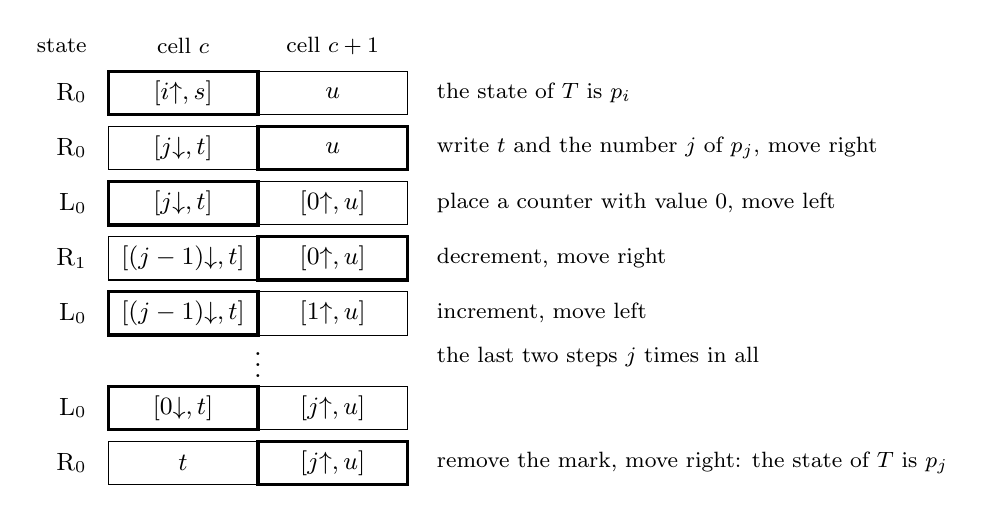
\begin{tikzpicture}[x=1mm,y=1mm,cell/.style={draw,minimum width=19mm,minimum height=5.5mm,inner sep=1pt,font=\small}]
\def\tmrow#1#2#3#4#5#6{%
  \node[anchor=east,font=\small] at (-1,#1) {$#2$};
  \node[cell] at (10,#1) {$#3$};
  \node[cell] at (29,#1) {$#4$};
  \ifnum#5=0 \draw[very thick] (0.5,{#1-2.75}) rectangle (19.5,{#1+2.75});\else \draw[very thick] (19.5,{#1-2.75}) rectangle (38.5,{#1+2.75});\fi
  \node[anchor=west,font=\footnotesize] at (41,#1) {#6};}
\node[font=\footnotesize] at (10,6) {cell $c$};
\node[font=\footnotesize] at (29,6) {cell $c+1$};
\node[font=\footnotesize,anchor=east] at (-1,6) {state};
\tmrow{0}{\mathrm{R}_0}{[i{\uparrow},s]}{u}{0}{the state of $T$ is $p_i$}
\tmrow{-7}{\mathrm{R}_0}{[j{\downarrow},t]}{u}{1}{write $t$ and the number $j$ of $p_j$, move right}
\tmrow{-14}{\mathrm{L}_0}{[j{\downarrow},t]}{[0{\uparrow},u]}{0}{place a counter with value 0, move left}
\tmrow{-21}{\mathrm{R}_1}{[(j-1){\downarrow},t]}{[0{\uparrow},u]}{1}{decrement, move right}
\tmrow{-28}{\mathrm{L}_0}{[(j-1){\downarrow},t]}{[1{\uparrow},u]}{0}{increment, move left}
\node at (19.5,-33.5) {$\vdots$};
\node[anchor=west,font=\footnotesize] at (41,-33.5) {the last two steps $j$ times in all};
\tmrow{-40}{\mathrm{L}_0}{[0{\downarrow},t]}{[j{\uparrow},u]}{0}{}
\tmrow{-47}{\mathrm{R}_0}{t}{[j{\uparrow},u]}{1}{remove the mark, move right: the state of $T$ is $p_j$}
\end{tikzpicture}
\caption{Morita's four-state conversion executing a right-moving quintuple $[p_i,s,t,\mathrm{R},p_j]$}
\label{fig:four}
\end{figure}

\paragraph{Disjoint ranges by direction.}
Number the states of $Q_+$ by $1,\dots,m_+$ and those of $Q_-$ by $m_++1,\dots,m$.
The converted machine has the four states $H_+,H_-,A_+,A_-$, where the index is the direction by which the state is entered, and its symbols are the plain symbols $s$ and the counter symbols $[i,s]$.
A \emph{stable} ID has exactly one counter symbol, under the head, and the machine in an $H$-state; it represents the ID of $T$ obtained by replacing $[i,s]$ by $s$ and taking the state numbered $i$.
For a quintuple $[p,s,t,D,q]$ of $T$ with $p\in Q_e$, the converted machine uses the rules
\begin{center}
\small
\begin{tabular}{llllll}
\toprule
& state & read & write & move & next \\
\midrule
R1 & $H_e$ & $[\nu(p),s]$ & $[\nu(q),t]$ & $D$ & $H_D$ \\
R2 & $H_D$ & $s'$ & $[\ell_D,s']$ & $\bar D$ & $A_{\bar D}$ \\
R3 & $A_{\bar D}$ & $[i,x]$, $\ell_D<i\le h_D$ & $[i-1,x]$ & $D$ & $A_D$ \\
R4 & $A_{\bar D}$ & $[\ell_D,x]$ & $x$ & $D$ & $H_D$ \\
R5 & $A_D$ & $[j,s']$, $\ell_D\le j<h_D$ & $[j+1,s']$ & $\bar D$ & $A_{\bar D}$ \\
\bottomrule
\end{tabular}
\end{center}
where $\nu$ is the numbering, $[\ell_D,h_D]$ is the range of numbers of $Q_D$, and $\bar D$ is the direction opposite to $D$.
The sum of the two counters is invariant during the back-and-forth phase, and R4 fires exactly when the whole number has been carried, so a stable ID is restored after $3+2(\nu(q)-\ell_D)$ steps.
The state $A_+$ acts as the target side of a right move and as the source side of a left move, but the counter values it reads in the two roles lie in disjoint ranges, so the table is deterministic; reversibility follows by the same separation together with the reversibility of $T$.
The marks are no longer needed, and the number of symbols becomes $(m+1)n$.
From URTM$(10,8)$ this gives four states and 88 symbols.

\paragraph{Reverse counting.}
If the counters are counted in opposite directions for the two directions of motion (the sentinel of $Q_+$ at the smallest value and that of $Q_-$ at the largest), then the decrement rule R3 of one direction and the increment rule R5 of the other become literally the same quintuple.
The two directions can then share one range of values, and the number of symbols is at most $(\max(m_+,m_-)+1)n$.
Figure~\ref{fig:ranges} compares the two numberings.
\begin{figure}[tb]
\centering
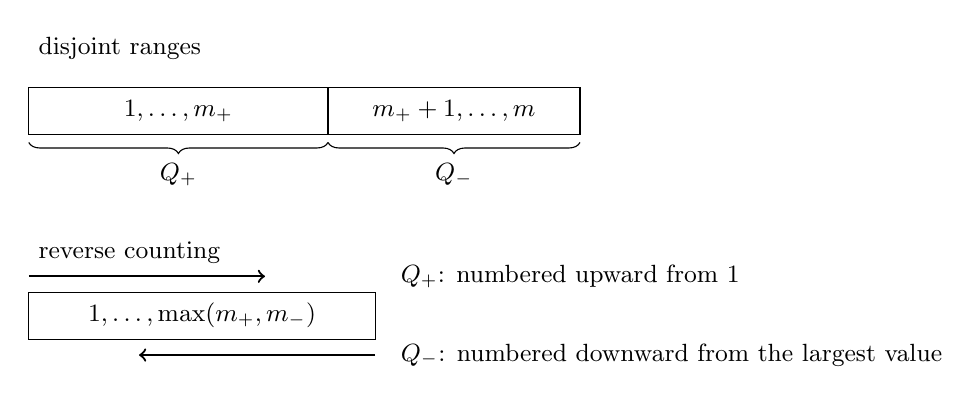
\begin{tikzpicture}[x=1mm,y=1mm,font=\small]
\node[anchor=west] at (0,8) {disjoint ranges};
\draw (0,-3) rectangle (70,3); \draw (38,-3) -- (38,3);
\node at (19,0) {$1,\dots,m_+$}; \node at (54,0) {$m_++1,\dots,m$};
\draw[decorate,decoration={brace,mirror,amplitude=4pt}] (0,-4) -- (38,-4) node[midway,below=4pt] {$Q_+$};
\draw[decorate,decoration={brace,mirror,amplitude=4pt}] (38,-4) -- (70,-4) node[midway,below=4pt] {$Q_-$};
\node[anchor=west] at (0,-18) {reverse counting};
\draw (0,-29) rectangle (44,-23);
\node at (22,-26) {$1,\dots,\max(m_+,m_-)$};
\draw[->,thick] (0,-21) -- (30,-21);
\node[anchor=west] at (46,-21) {$Q_+$: numbered upward from 1};
\draw[->,thick] (44,-31) -- (14,-31);
\node[anchor=west] at (46,-31) {$Q_-$: numbered downward from the largest value};
\end{tikzpicture}
\caption{Counter values of the states of $Q_+$ and $Q_-$ in the four-state conversions}
\label{fig:ranges}
\end{figure}
From URTM$(10,8)$ this gives a reversible machine with four states and 48 symbols.
We prove that it simulates an arbitrary CTSH, but not that it is universal in the sense of Definition~\ref{def:univ}; it is dominated by URTM$(4,42)$ in any case.

\subsection{Block decomposition and merging of roles}
\label{sec:blocks}

Split the number of a state into a pair (block, value within the block).
The finite control holds the block and the tape holds only the value, so a counter symbol $[i,s]$ does not record the block, and different blocks reuse the same values.
With $b_+$ blocks for $Q_+$ and $b_-$ blocks for $Q_-$, each block $\beta$ has three roles: $H_\beta$ (stable), $O_\beta$ (the source side of a carry), and $D_\beta$ (the target side of a carry).
The rules are those of Section~\ref{sec:four} with block indices; R1 goes from $H_{\mathrm{blk}(p)}$ to $H_{\mathrm{blk}(q)}$.
The roles still have to know their block in the back-and-forth phase, because R4 must enter the correct $H$-state; this is what costs states.
Figure~\ref{fig:blocks} shows the splitting for seven states in two blocks.
\begin{figure}[tb]
\centering
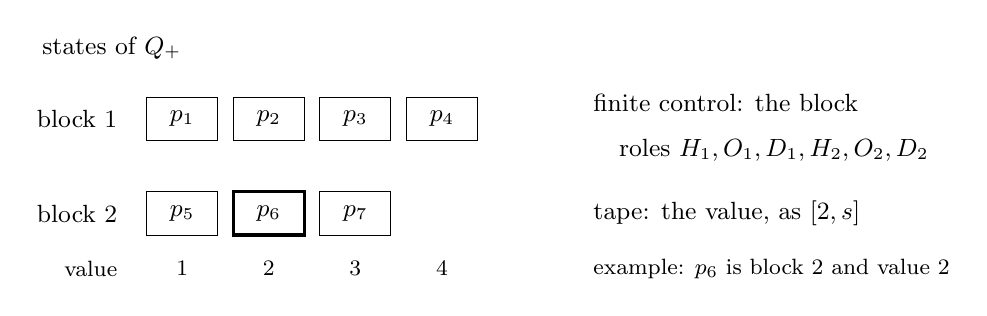
\begin{tikzpicture}[x=1mm,y=1mm,font=\small,st/.style={draw,minimum width=9mm,minimum height=5.5mm,inner sep=1pt}]
\node[anchor=west] at (-14,9) {states of $Q_+$};
\node[anchor=east] at (-2,0) {block 1};
\node[anchor=east] at (-2,-12) {block 2};
\foreach \k in {1,...,4} \node[st] at ({(\k-1)*11+5},0) {$p_{\k}$};
\foreach \k/\v in {5/1,6/2,7/3} \node[st] at ({(\v-1)*11+5},-12) {$p_{\k}$};
\foreach \v in {1,...,4} \node[font=\footnotesize] at ({(\v-1)*11+5},-19) {$\v$};
\node[anchor=east,font=\footnotesize] at (-2,-19) {value};
\draw[very thick] (11.5,-14.75) rectangle (20.5,-9.25);
\node[anchor=west] at (56,2) {finite control: the block};
\node[anchor=west] at (56,-4) {\quad roles $H_1,O_1,D_1,H_2,O_2,D_2$};
\node[anchor=west] at (56,-12) {tape: the value, as $[2,s]$};
\node[anchor=west,font=\footnotesize] at (56,-19) {example: $p_6$ is block 2 and value 2};
\end{tikzpicture}
\caption{Splitting the numbers of the states of $Q_+$ into blocks and values (an example with seven states)}
\label{fig:blocks}
\end{figure}

A \emph{merging of roles} is a partition of the roles into classes; each class becomes one state.
Roles in the same class must be entered from the same direction, and the merged table must remain deterministic and reversible.
The reverse-counting trick of Section~\ref{sec:four} is the special case where the source role of one direction and the target role of the other are merged in a single block.
A further merging that turned out to be useful puts a single state into a block of its own, gives it a counter value outside the range of the main blocks, and merges its $H$-role into a back-and-forth state of a main block; then a counter value outside the main range alone signals that the machine is in that state, and no carry is needed.

Only the counter symbols that can actually occur are kept.
If $V$ is the set of counter values used and $X_i$ is the set of original symbols that can carry the value $i$, the number of symbols is
\[
  n+\sum_{i\in V}|X_i|\ \le\ (|V|+1)n .
\]
The choice of the blocks, of the values, and of the merging is a combinatorial optimization problem.
We solved it with a constraint programming model (one Boolean variable for each state, block, and value, with determinism and reversibility as constraints on the generated rules) and with simulated annealing over the partitions.
This gives URTM$(4,46)$ from $(10,8)$, for example, with $V=\{1,2,3,4,6\}$: the main blocks use the values 1 to 4, and two states placed in blocks of their own share the value 6.
Table~\ref{tab:blocks} lists the six machines with four to nine states obtained in this way.
They are all dominated by the machines of Section~\ref{sec:merge}, but they are universal in their own right, and they are the inputs to symbol merging.
The book contains no conversion that produces five to nine states.

\begin{table}[tb]
\centering
\caption{Machines obtained by block decomposition and merging of roles}
\label{tab:blocks}
\small
\begin{tabular}{llllrr}
\toprule
Point & Original & $V$ & $|X_i|$ for $i\in V$ & $n+\sum|X_i|$ & $(|V|+1)n$ \\
\midrule
$(4,46)$ & $(10,8)$ & $\{1,2,3,4,6\}$ & 8, 8, 8, 8, 6 & 46 & 48 \\
$(5,45)$ & $(15,6)$ & $\{1,\dots,8\}$ & 3, 5, 5, 5, 5, 5, 5, 6 & 45 & 54 \\
$(6,37)$ & $(10,8)$ & $\{1,2,5,6\}$ & 6, 7, 8, 8 & 37 & 40 \\
$(7,32)$ & $(15,6)$ & $\{1,\dots,5\}$ & 6, 5, 5, 5, 5 & 32 & 36 \\
$(8,28)$ & $(17,5)$ & $\{2,4,5,6,7\}$ & 3, 5, 5, 5, 5 & 28 & 30 \\
$(9,27)$ & $(15,6)$ & $\{1,2,3,4\}$ & 6, 5, 5, 5 & 27 & 30 \\
\bottomrule
\end{tabular}
\end{table}

\begin{remark}
Three states cannot be reached in this framework, which merges neither two $H$-roles nor the $H$- and $D$-roles of the same block.
If $Q_-$ has at least two states, then either some block of $Q_-$ has two or more states, and its $H$- and $D$-roles fall into different classes, or there are two single-state blocks with two $H$-roles.
In either case the roles entered from the left need at least two classes.
The same holds for $Q_+$, so at least four states are needed for all six of Morita's machines.
\end{remark}

\subsection{Symbol merging}
\label{sec:merge}

In a converted table, each counter symbol is read by few states and written into few states.
Kudlek and Rogozhin reduced a standard UTM by identifying the blank with another symbol~\cite{KudlekRogozhin02}.
We apply the same idea systematically.
Two symbols $x$ and $y$ \emph{conflict} if some state reads both, some state is entered by quintuples writing $x$ and $y$, or both can occur on the tape of a halting ID reached from an encoded input.
Merging pairwise non-conflicting symbols is a coloring of the conflict graph: symbols of the same color become one symbol.
The merged table is deterministic and reversible if the original is, and it follows the run of the original step by step.

The general statement that we prove is the following.

\begin{theorem}[Symbol merging]
\label{thm:merge}
Let $U$ satisfy $\mathrm{IsUTMStrict}(U)$, and assume that every halting ID reached from an encoded input is in a state that is not a source state and has all its tape symbols in a fixed finite set $F$.
Let $h,\rho:\mathbb{N}\to\mathbb{N}$ be primitive recursive with $h(0)=\rho(0)=0$ and $\rho(h(x))=x$ for every $x\in F$.
If the table $h(U)$, obtained by replacing the read and written symbols of every quintuple by their images under $h$, is deterministic, then $\mathrm{IsUTMStrict}(h(U))$.
\end{theorem}

Here $h$ is the coloring and $\rho$ recovers the original symbols on halting tapes; the hypothesis on the halting states holds because, in runs from encoded inputs, our block tables halt only by entering a halting state.
Applied to the fixed tables of Table~\ref{tab:blocks}, merging removes one to three symbols.
Much more is gained by choosing the blocks and values again, by simulated annealing, with the number of colors after merging as the objective.
All five best results come from URTM$(13,7)$ (Table~\ref{tab:merge}).
We do not claim minimality, either of the coloring or over the choices of blocks.

\begin{table}[tb]
\centering
\caption{Machines obtained by symbol merging}
\label{tab:merge}
\small
\begin{tabular}{llcrr}
\toprule
Point & Original & Blocks $(b_+,b_-)$ & Symbols before merging & Symbols after merging \\
\midrule
$(4,42)$ & $(13,7)$ & $(2,2)$ & 50 & 42 \\
$(5,39)$ & $(13,7)$ & $(3,2)$ & 49 & 39 \\
$(6,30)$ & $(13,7)$ & $(3,3)$ & 54 & 30 \\
$(7,28)$ & $(13,7)$ & $(4,3)$ & 50 & 28 \\
$(8,21)$ & $(13,7)$ & $(4,4)$ & 40 & 21 \\
\bottomrule
\end{tabular}
\end{table}

\subsection{Three states}
\label{sec:three}

Morita's conversion to three states~\cite[Sect.~5.3.5]{Morita17} has two stages.
Lemma~5.9 turns $T$ into a \emph{one-way-updating} RTM $\hat T$, which rewrites the tape only while sweeping to the right and returns to the left end in a single state without rewriting.
Its tape packs two cells of $T$ into one cell, with $N=mn^2+n^2+1$ symbols (the blank, the pairs, and the pairs marked with a state), and it has $M=m_+n+2n+2$ states.
Lemma~5.10 then represents the state $q_i$ of $\hat T$ by a counter $[x,i]$ with an up or a down mark on the symbol under the head and uses three states $\rmL$, $\rmR_0$, $\rmR_1$, which gives $N(2M-1)$ symbols.
From URTM$(32,3)$ this is URTM$(3,36654)$.
Of these symbols, 85\% are counters that combine a marked pair, one of the $m_+n$ states of $\hat T$ entered after a right move, and an up or down mark.
We reduce the count in four steps.

\paragraph{Shared counters.}
In a one-way-updating machine all carries go to the right, so each of the three states always reads counters on a fixed side: $\rmL$ only on the source side, $\rmR_0$ and $\rmR_1$ only on the target side.
Hence the up and down marks can be identified without losing determinism, and reversibility is preserved, since the written symbols of the rules entering each state remain distinct.
The count drops from $N(2M-1)$ to $NM$, that is, from 36,654 to 18,476 for $(32,3)$.

\paragraph{Pruned counters.}
A counter $[x,k]$ is needed only if some state with number at least $k$ can read $x$ or is entered by writing $x$.
Keeping only these counters gives $N+\sum_x\mathrm{need}(x)$ symbols, where $\mathrm{need}(x)$ is the largest such number.
The sum depends on the numbering of the states of $\hat T$; states with the same set of relevant symbols can be kept adjacent, and the best order of these groups gives 1,820 symbols for $(32,3)$.
The machines with 18,476 and 1,820 symbols only measure the effect of these two steps: we count their symbols but do not prove that they simulate $T$, and for the second one we do not show that the kept counters suffice along every run.
Universality is proved for the machines of the next two steps.

\paragraph{One symbol per cell.}
The remaining cost lies in the $n^2$ pairs and the $mn^2$ marked pairs.
Morita packs two cells to distinguish the blank of $T$ from the blank of $\hat T$ and to extend the used region one cell at a time.
We instead keep one symbol per cell and represent the blank of $T$ by a separate symbol $B$ inside the used region.
The sweep shifts the whole content of $T$ one cell to the right, as in Morita's construction, so a left move of $T$ does not overshoot its target.
The current state $p$ of $T$ is recorded as a mark on one cell: on the head cell if $p\in Q_-$, and on the cell to the left of the head if $p\in Q_+$.
The one-way-updating machine has $n+3+|R|+|G|$ states, where $R$ is the set of pairs $(q,t)$ such that $T$ has a right-moving quintuple into $q$ writing $t$, and $G=R\cup(\{p_0\}\times S)$ if the initial state $p_0$ is in $Q_+$ and $G=R$ otherwise ($S$ is the set of symbols of $T$).
After the shared and pruned counters, the three-state machine has
\[
  1+n+(m_-n+|G|)(n+1)+n(n+2+|R|+|G|)+(n+2)
\]
symbols.
Since $|R|\le\min(|\delta|,m_+n)$, where $|\delta|$ is the number of quintuples of $T$, this is $O(n(mn+|\delta|))\subseteq O(mn^2)$, compared with $O(m\,m_+n^3)$ for Morita's construction.
For $(32,3)$ it gives 659 symbols.

\paragraph{Reflection.}
Applying the conversion to the mirror image of $T$ (directions L and R exchanged) and mirroring the result back exchanges the roles of $m_+$ and $m_-$ and of the right-moving and left-moving targets.
For $(32,3)$ this gives 600 symbols, and hence URTM$(3,600)$.
Applied to the other five original machines, the improved conversion gives between 802 and 1,209 symbols (with or without reflection), so $(32,3)$ is the best starting point.

\subsection{Two symbols}
\label{sec:two}

Morita's conversion to two symbols~\cite[Sect.~5.3.3]{Morita17} replaces each symbol by a $k$-bit block, the blank by $0^k$.
A quintuple of $T$ is simulated by reading $k-1$ bits while erasing them, reading the last bit and writing the last bit of the new symbol, writing the remaining bits while moving back, and moving $k-1$ cells in the direction of the move; the states remember the prefix read or the prefix still to write.
If $P_r$ and $P_w$ denote the numbers of read and written prefixes of lengths 1 to $k-1$, summed over the states, the number of states is at most $mk+P_r+P_w$.
From URTM$(24,4)$ ($k=2$) this gives URTM$(138,2)$, and from URTM$(13,7)$ ($k=3$) it gives 169 states.

We add four degrees of freedom: the assignment of codes to symbols (the blank fixed to $0^k$), the values written in place of the bits that have been read, a path type for each quintuple that says how many bits need not be rewritten on the way back (a right-moving quintuple can then cross its block once instead of three times), and, for each state, the end of the block at which the head stands when reading begins.
Reversibility of the result reduces to distinct written values on the rules entering each auxiliary state.
For fixed codes and orientations, the written values and the path types are chosen by a constraint programming model that minimizes the number of auxiliary states; the codes and orientations are chosen by exhaustive enumeration and hill climbing.
Finally, states with the same behavior are merged; a merged table fills undefined entries of one state with the rules of the other, so it simulates $T$ only along runs that never halt in an undefined entry, which is the case for runs from encoded CTSH inputs.
For $(13,7)$ the steps give 149, 135, and 92 states.
A randomized large-neighborhood search over the choices of the table before merging then gave a table with 137 states that merges down to 85 states and 153 quintuples, that is, URTM$(85,2)$.
We have no closed formula for the size of this search result; it is verified for the concrete table.
Applied to the other five original machines, the same method, including the search, gives 92, 92, 108, 115, and 115 states for $(10,8)$, $(24,4)$, $(15,6)$, $(17,5)$, and $(32,3)$.
These five tables are also proved universal in the sense of Definition~\ref{def:univ}, and all of them are dominated by URTM$(85,2)$.

\section{The new URTMs and their universality}
\label{sec:univ}

\begin{theorem}[Existence]
\label{thm:exists}
For each of the 13 points
\begin{multline*}
(m,n)\in\{(3,600),(4,42),(5,39),(6,30),(7,28),(8,21),(10,8),\\(13,7),(15,6),(17,5),(24,4),(32,3),(85,2)\},
\end{multline*}
there is a table $U$ that is deterministic and reversible, satisfies $\mathrm{NStates}(U)=m$ and $\mathrm{NSyms}(U)=n$, and satisfies $\mathrm{IsUTMStrict}(U)$.
\end{theorem}

Figure~\ref{fig:compare} places these points among the known ones.
The six points from $(10,8)$ to $(32,3)$ are Morita's original machines, which remain non-dominated; the other seven are new.
The witnesses are concrete rule tables: Morita's distributed tables~\cite{MoritaFiles} and the tables produced from them by the conversions of Section~\ref{sec:constr}.

\begin{figure}[tb]
\centering
\resizebox{\textwidth}{!}{%
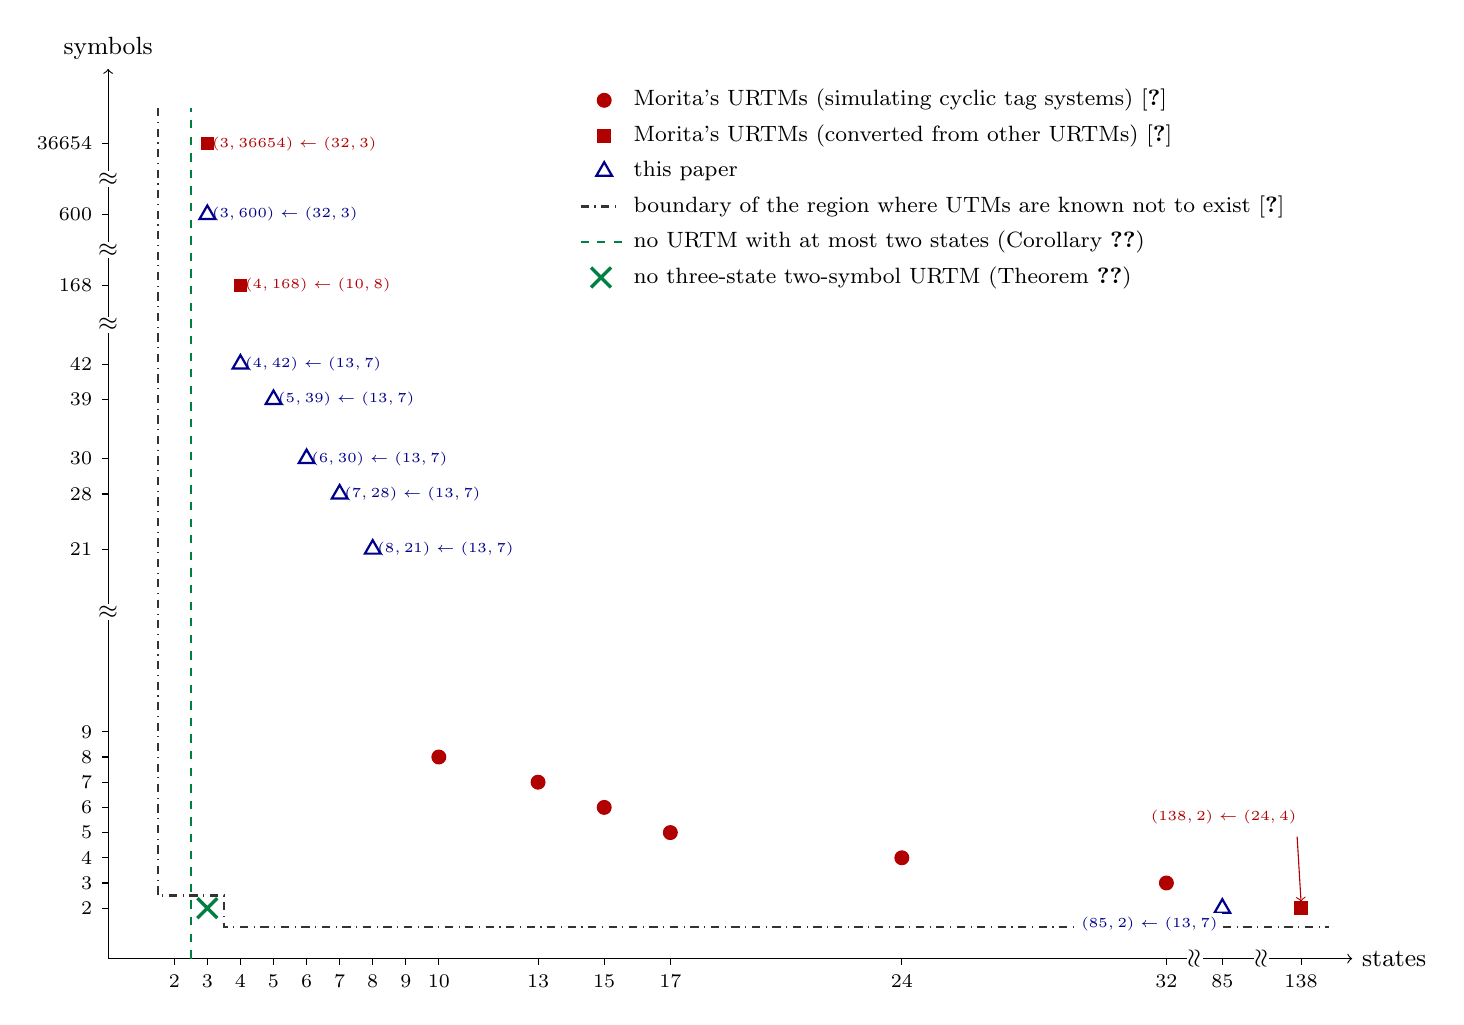
\begin{tikzpicture}[font=\scriptsize,
  wave/.style={fill=white, inner sep=0.6pt, font=\small}]
\definecolor{cM}{RGB}{176,0,0}\definecolor{cU}{RGB}{0,0,140}\definecolor{cO}{RGB}{0,128,64}
\draw[->] (0,0) -- (15.8,0) node[anchor=west,font=\small] {states};
\draw[->] (0,0) -- (0,11.3) node[anchor=south,font=\small] {symbols};
\foreach \x/\l in {0.840/2,1.260/3,1.680/4,2.100/5,2.520/6,2.940/7,3.360/8,3.780/9,4.200/10,5.460/13,6.300/15,7.140/17,10.080/24,13.440/32,14.150/85,15.150/138}
  \draw (\x,0) -- (\x,-0.08) node[below] {\l};
\foreach \y/\l in {0.640/2,0.960/3,1.280/4,1.600/5,1.920/6,2.240/7,2.560/8,2.880/9,5.200/21,5.900/28,6.350/30,7.100/39,7.550/42,8.550/168,9.450/600,10.350/36654}
  \draw (0,\y) -- (-0.08,\y) node[left] {\l};
\node[wave,rotate=90] at (13.800,0) {$\approx$};
\node[wave,rotate=90] at (14.650,0) {$\approx$};
\node[wave] at (0,4.400) {$\approx$};
\node[wave] at (0,8.050) {$\approx$};
\node[wave] at (0,9.000) {$\approx$};
\node[wave] at (0,9.900) {$\approx$};
\draw[dashed, cO, thick] (1.050,0) -- (1.050,10.800);
\draw[black!80, dash dot, thick] (0.630,10.800) -- (0.630,0.800) -- (1.470,0.800) -- (1.470,0.400) -- (15.500,0.400);
\node[cross out,draw=cO,very thick,inner sep=0pt,minimum size=6pt] at (1.260,0.640) {};
\foreach \x/\y in {4.200/2.560,5.460/2.240,6.300/1.920,7.140/1.600,10.080/1.280,13.440/0.960}
  \node[circle,draw=cM,fill=cM,inner sep=0pt,minimum size=5pt] at (\x,\y) {};
\foreach \x/\y in {15.150/0.640,1.680/8.550,1.260/10.350}
  \node[rectangle,draw=cM,fill=cM,inner sep=0pt,minimum size=4.5pt] at (\x,\y) {};
\foreach \x/\y in {1.260/9.450,1.680/7.550,2.100/7.100,2.520/6.350,2.940/5.900,3.360/5.200,14.150/0.640}
  \node[regular polygon,regular polygon sides=3,draw=cU,fill=white,thick,inner sep=0pt,minimum size=6.5pt] at (\x,\y) {};
\node[anchor=west,font=\tiny,text=cM,inner sep=1.5pt] at (1.260,10.350) {$(3,36654)\leftarrow(32,3)$};
\node[anchor=west,font=\tiny,text=cM,inner sep=1.5pt] at (1.680,8.550) {$(4,168)\leftarrow(10,8)$};
\node[anchor=south east,font=\tiny,text=cM,fill=white,inner sep=1.5pt] at (15.150,1.650) {$(138,2)\leftarrow(24,4)$};
\draw[->,cM,thin] (15.100,1.550) -- (15.150,0.720);
\node[anchor=west,font=\tiny,text=cU,inner sep=1.5pt] at (1.260,9.450) {$(3,600)\leftarrow(32,3)$};
\node[anchor=west,font=\tiny,text=cU,inner sep=1.5pt] at (1.680,7.550) {$(4,42)\leftarrow(13,7)$};
\node[anchor=west,font=\tiny,text=cU,inner sep=1.5pt] at (2.100,7.100) {$(5,39)\leftarrow(13,7)$};
\node[anchor=west,font=\tiny,text=cU,inner sep=1.5pt] at (2.520,6.350) {$(6,30)\leftarrow(13,7)$};
\node[anchor=west,font=\tiny,text=cU,inner sep=1.5pt] at (2.940,5.900) {$(7,28)\leftarrow(13,7)$};
\node[anchor=west,font=\tiny,text=cU,inner sep=1.5pt] at (3.360,5.200) {$(8,21)\leftarrow(13,7)$};
\node[anchor=north east,font=\tiny,text=cU,fill=white,inner sep=1.5pt] at (14.150,0.580) {$(85,2)\leftarrow(13,7)$};
\node[circle,draw=cM,fill=cM,inner sep=0pt,minimum size=5pt] at (6.300,10.900) {};
\node[anchor=west,font=\footnotesize] at (6.55,10.90) {Morita's URTMs (simulating cyclic tag systems)~\cite{Morita17}};
\node[rectangle,draw=cM,fill=cM,inner sep=0pt,minimum size=4.5pt] at (6.300,10.450) {};
\node[anchor=west,font=\footnotesize] at (6.55,10.45) {Morita's URTMs (converted from other URTMs)~\cite{Morita17}};
\node[regular polygon,regular polygon sides=3,draw=cU,fill=white,thick,inner sep=0pt,minimum size=6.5pt] at (6.300,10.000) {};
\node[anchor=west,font=\footnotesize] at (6.55,10.00) {this paper};
\draw[black!80, dash dot, thick] (6.000,9.550) -- (6.520,9.550);
\node[anchor=west,font=\footnotesize] at (6.55,9.55) {boundary of the region where UTMs are known not to exist~\cite{WoodsNeary09}};
\draw[dashed,cO,thick] (6.000,9.100) -- (6.520,9.100);
\node[anchor=west,font=\footnotesize] at (6.55,9.10) {no URTM with at most two states (Corollary~\ref{cor:twostate})};
\node[cross out,draw=cO,very thick,inner sep=0pt,minimum size=6pt] at (6.260,8.650) {};
\node[anchor=west,font=\footnotesize] at (6.55,8.65) {no three-state two-symbol URTM (Theorem~\ref{thm:threetwo})};
\end{tikzpicture}}
\caption{Numbers of states and symbols of URTMs}
\label{fig:compare}
\end{figure}

The dash-dotted line in Figure~\ref{fig:compare} bounds the region where UTMs are known not to exist~\cite{WoodsNeary09}: one-state machines, two-state and three-state two-symbol machines (under a definition that reserves one transition for halting), and one-symbol machines.
These results concern TMs that need not be reversible, and their treatment of halting and of zero-shifts differs from ours, so we do not use them for URTMs in our sense.
The green lines mark our own nonexistence results (Sections~\ref{sec:twostate} and~\ref{sec:threetwo}), which are stated for the same notion of universality as Theorem~\ref{thm:exists}.

\subsection{Proof of universality}

Each witness other than the five merged ones is first shown to simulate an arbitrary CTSH: for every CTSH $\hat C$ and initial string $v$, the machine started on the code of $(\hat C,v)$ halts if and only if $\hat C$ halts from $(v,0)$, and its halting ID is the code of the halting ID of $\hat C$.
For Morita's six machines this is a direct proof about the given tables.
For the converted machines it follows from general simulation theorems for the conversions (preservation of determinism, reversibility, one-step simulation, and the correspondence of halting, halting IDs, and non-halting), instantiated with the concrete tables.
The five merged machines inherit universality from their tables before merging by Theorem~\ref{thm:merge}.

Universality in the sense of Definition~\ref{def:univ} then requires computable maps between arbitrary TMs and CTSHs.
We formalize the chain
\[
  \mathrm{tm}(i)\ \longrightarrow\ \text{two-register machine}\ \longrightarrow\ \text{2-tag system}\ \longrightarrow\ \text{CTSH}\ \longrightarrow\ U,
\]
which follows the classical route of Cocke and Minsky~\cite{CockeMinsky64} and Morita's Theorem~7.2.
The first step stores the tape of $\mathrm{tm}(i)$ in two registers and normalizes the symbols of $\mathrm{tm}(i)$, which are arbitrary natural numbers, into binary; this replaces a separate conversion of the TM to two symbols.
A general theorem then states that a machine that simulates an arbitrary CTSH and has a primitive recursive input encoding and a primitive recursive readout of the final string, independent of trailing blanks, satisfies $\mathrm{IsUTMStrict}$.
Each machine supplies only its numbering, encoding, and readout.

\begin{proposition}[Agreement]
Let $U_1$ and $U_2$ be deterministic tables satisfying $\mathrm{IsUTMStrict}$ with encodings $c_1,c_2$ and decodings $d_1,d_2$.
For every TM $\mathrm{tm}(i)$ and admissible input $a$, $U_1$ halts from $\mathrm{toID}(0,c_1(i,a))$ if and only if $U_2$ halts from $\mathrm{toID}(0,c_2(i,a))$, and if both halt, the decoded halting IDs are equal.
In particular this holds for any two of the 13 witnesses of Theorem~\ref{thm:exists}.
\end{proposition}

The encoded inputs, the runs, and the numbers of steps differ between machines; only halting and the decoded result agree.

\paragraph{Halting quintuples.}
For the 11 points other than $(85,2)$ and $(3,600)$, the distributed tables represent the halting entries of the book by two zero-shift quintuples into halting states that are not counted.
We prove Theorem~\ref{thm:exists} also for the tables without these two quintuples, which are the tables printed in the book or, for the five merged points, their analogues.
Removing them changes neither the number of states nor the number of symbols; the decoder first maps the halting ID back to the corresponding halting state.

\subsection{Counting states and symbols}
\label{sec:counting}

Morita does not count halting states in the $m$ of URTM$(m,n)$.
The book states that the set of final states is not specified in the problem of reducing the number of states, the state sets of the URTMs in Chapter~7 contain no halting states, and in Chapter~11 it notes that the halting states are not included in URTM$(17,5)$~\cite{Morita17}.
The distributed files also state explicitly that the halting states are not counted.

Our $\mathrm{NStates}$ counts source states and $\mathrm{NSyms}$ counts the symbols occurring in the table together with the blank.
The two conventions could differ for states that occur only as targets, for halting states, and for symbols that do not occur in the table.
For the witness tables of Theorem~\ref{thm:exists} we prove that every target is a source state; for $(85,2)$ and $(3,600)$ this holds already for the tables in the form of the distributed files, and for the other 11 points it holds for the tables without the two halting quintuples.
Hence the number of states remains $m$ even under a convention that also counts targets.
We also prove that the blank occurs in each witness and that every symbol is both read and written, and that the witnesses have exactly $(m,n)$ under Morita's way of counting (targets counted, only symbols occurring in the table).
An independent count outside the proof assistant agrees (Table~\ref{tab:counts}).
For the 11 distributed tables with the additional halting quintuples, counting targets gives $m+2$ states.

\begin{table}[tb]
\centering
\caption{Independent count of states and symbols in the witness tables}
\label{tab:counts}
\small
\begin{tabular}{lrcccc}
\toprule
Table & Quint. & Sources & Target-only & Symbols & Zero-shifts \\
\midrule
Morita's 6 points, distributed & 59--84 & $m$ & 2 & $n$ & 2 \\
same, tables in the book & 57--82 & $m$ & 0 & $n$ & 0 \\
5 symbol-merging points, distributed & 143--162 & $m$ & 2 & $n$ & 2 \\
same, without 2 quintuples & 141--160 & $m$ & 0 & $n$ & 0 \\
$(85,2)$ & 153 & 85 & 0 & 2 & 0 \\
$(3,600)$ & 1,572 & 3 & 0 & 600 & 0 \\
\bottomrule
\end{tabular}
\end{table}

\section{Nonexistence of URTMs with at most two states}
\label{sec:twostate}

\begin{theorem}[Halting of two-state RTMs]
\label{thm:halting}
There is a computable Boolean function $f$ such that, for all distinct states $q_0,q_1,q_f$, every deterministic and reversible table $T$ whose source states are among $q_0,q_1$ and whose targets are among $q_0,q_1,q_f$, every position $p\in\mathbb{Z}$, and every code $z\in\Code$,
\[
  f(T,p,z)=\mathrm{true}\iff\mathrm{Halts}_T(\mathrm{toID}(p,z)).
\]
\end{theorem}

\begin{corollary}
\label{cor:twostate}
If $U$ is deterministic and reversible and $\mathrm{NStates}(U)\le 2$, then $\neg\mathrm{IsUTM}(U)$, and hence $\neg\mathrm{IsUTMStrict}(U)$.
Moreover, there is a TM $\mathrm{tm}(i)$ that no deterministic and reversible two-state table simulates in the sense of conditions~2 and~3 of Definition~\ref{def:univ}.
\end{corollary}

The corollary follows from Theorem~\ref{thm:halting} and the undecidability of the halting problem.
Two reductions bring a general table into the form of the theorem.
A one-state table is a special case of a two-state one.
If a table has several halting targets, removing the quintuples whose target is not a source state does not change whether the machine halts: if the original run halts by executing a removed quintuple, the reduced run halts one step earlier.
Removing quintuples preserves determinism and reversibility.
The corollary therefore holds for any number of symbols, and with zero-shifts and halting states allowed as in Morita's definition.
If this formalization captures Morita's Definition~7.1, it answers the question of the book and of the survey~\cite{Morita23} negatively.

\paragraph{Proof outline of Theorem~\ref{thm:halting}.}
Let $T$ be as in the theorem, with the quintuples into $q_f$ removed.
Fix an initial finite ID and a window $[a,b]$ containing its non-blank cells and its head; let $w=b-a+1$ and let $n$ be the number of symbols.

\begin{enumerate}
\item \emph{The state is the direction of the last move.}
By the unique shift-direction property, if $T$ has both a left-moving and a right-moving quintuple, then one state is entered only by left moves, the other only by right moves, and there is no zero-shift.
So the state records the direction of the last move, and $T$ is a partial injection $\pi:\{\rmL,\rmR\}\times\Sigma\rightharpoonup\Sigma\times\{\rmL,\rmR\}$.
(If $T$ moves in only one direction, the head enters blank cells beyond the window in one of two states, so a state repeats by the third such cell, the run repeats itself shifted, and it does not halt; a halting run is therefore short.)
\item \emph{A half-line reports only that the head came back.}
Fix a boundary and the half-line $H$ to its right.
The head always enters $H$ in state R and leaves it in state L, and the behavior inside $H$ does not depend on the content outside.
Hence the outcome of the $j$-th entry into $H$ (leave, halt inside, or never return) and the content of $H$ on leaving depend only on the initial content of $H$ and on $j$.
Figure~\ref{fig:halfline} illustrates this.
\item \emph{The head cannot go deep into a blank half-line.}
Let $[k,\infty)$ be initially blank and consider a halting run.
The half-line $[k+1,\infty)$ is a translate of $[k,\infty)$, so by step~2 their contents at the $j$-th entry are translates of each other.
If the number of entries into $[k+1,\infty)$ caught up with that into $[k,\infty)$, the run would repeat itself shifted by one cell and never halt.
So the numbers of entries into $[k,\infty)$, $[k+1,\infty)$, $[k+2,\infty)$, \dots\ strictly decrease, and the head never passes $k$ plus the number of entries into $[k,\infty)$.
\item \emph{Each cell runs its own clock.}
A cell to the right of the initial head is first entered from the left, and afterwards the head can return only from the side to which it left.
So the pair (direction, symbol) at the $i$-th visit of the cell is obtained by iterating a fixed map $\kappa(d,s)=(\overline{d'},v)$, where $\pi(d,s)=(v,d')$, on a set of size $2n$.
All blank cells run the same clock, so a run that halts inside a blank half-line enters it at most $2n+1$ times.
\item \emph{Inside the window the machine is finite-state.}
Replacing each step that leaves the window by a turn at its end gives a machine with at most $Z=3w\,n^{w}$ configurations, whose orbit the real run follows inside the window by step~2.
A run that halts inside the window does so before the orbit becomes periodic; a run that halts in a half-line enters it in every period, hence by step~4 in boundedly many periods.
In both cases each half-line is entered at most $Z(2n+3)+1$ times.
\item \emph{A computable bound.}
By steps~3 and~5 the head of a halting run stays in a computable interval around the window.
A halting run of a deterministic machine never repeats an ID, so it halts within a number of steps bounded by a computable function of $n$ and $w$.
Running $T$ for that many steps decides halting.
\end{enumerate}
\begin{figure}[tb]
\centering
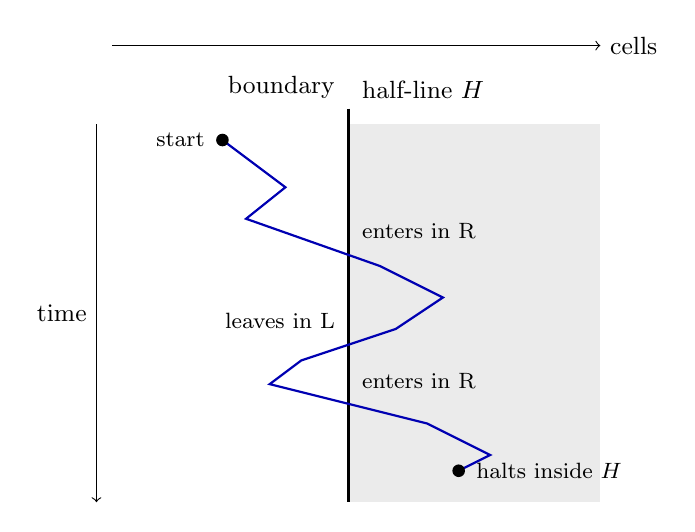
\begin{tikzpicture}[x=1mm,y=1mm,font=\small]
\fill[black!8] (30,2) rectangle (62,-46);
\draw[thick] (30,4) -- (30,-46);
\node[anchor=south east] at (29.5,4) {boundary};
\node[anchor=south west] at (30.5,4) {half-line $H$};
\draw[->] (-2,2) -- (-2,-46) node[midway,left] {time};
\draw[->] (0,12) -- (62,12) node[right] {cells};
\draw[thick,blue!70!black] (14,0) -- (22,-6) -- (17,-10) -- (34,-16) -- (42,-20) -- (36,-24) -- (24,-28) -- (20,-31) -- (40,-36) -- (48,-40) -- (44,-42);
\node[anchor=south west,font=\footnotesize] at (30.5,-13.8) {enters in R};
\node[anchor=south west,font=\footnotesize] at (30.5,-32.8) {enters in R};
\node[anchor=south east,font=\footnotesize] at (29.5,-25.2) {leaves in L};
\fill (14,0) circle (0.8);
\node[anchor=east,font=\footnotesize] at (13,0) {start};
\fill (44,-42) circle (0.8);
\node[anchor=west,font=\footnotesize] at (45,-42) {halts inside $H$};
\end{tikzpicture}
\caption{The head of a two-state RTM crossing the boundary of a half-line}
\label{fig:halfline}
\end{figure}
Only step~1 uses reversibility; steps~2 to~6 use only determinism and the fact that the state equals the direction of the last move.
In an irreversible two-state TM the same state can be entered from both sides, so a half-line can send more than one bit of information, and indeed such machines can be universal.
For three states, step~2 fails already for Morita's conversion to three states, which has two right-moving states.

\paragraph{Further nonexistence results.}
\begin{theorem}
\label{thm:onesym}
If $U$ is deterministic and $\mathrm{NSyms}(U)\le 1$, then $\neg\mathrm{IsUTM}(U)$, even if $U$ is not reversible.
\end{theorem}
The tape never changes, so a halting run halts within a bounded number of steps.

\begin{theorem}
\label{thm:oneL}
Let $U$ be deterministic and reversible with at most one left-moving quintuple $\ell$, and assume that no zero-shift quintuple has the source state of $\ell$ as its target.
Then $\neg\mathrm{IsUTM}(U)$.
The same holds with right and left exchanged.
\end{theorem}
This is a reversible counterpart of Pavlotskaya's theorem that the halting problem is decidable for two-symbol TMs with a single left-moving instruction~\cite{Pavlotskaya73}; here the number of states and symbols is arbitrary.
By reversibility, the only quintuple entering the target of $\ell$ is $\ell$ itself.

\section{Nonexistence of three-state two-symbol URTMs}
\label{sec:threetwo}

\begin{theorem}
\label{thm:threetwo}
Let $U$ be deterministic and reversible without repeated quintuples, and suppose there are distinct states $q_0,q_1,q_2$ and a symbol $\sigma\ne 0$ such that every quintuple of $U$ has its source state among $q_0,q_1,q_2$ and reads and writes only $0$ and $\sigma$.
Then $\neg\mathrm{IsUTMStrict}(U)$.
\end{theorem}

The formalized hypotheses are Boolean checks that compare every two entries at different positions of the list, so, unlike the definitions of Section~\ref{sec:prelim}, they also reject a table that lists the same quintuple twice.
Targets are arbitrary, so halting states and zero-shifts are allowed as in Morita's definition.
We first prove the theorem for Morita's formulation on string IDs, with the additional requirement that the encoded inputs use only the symbols $0$ and $\sigma$.
For deterministic two-symbol tables, $\mathrm{IsUTMStrict}$ implies this formulation, because the only symbols that occur are the blank and one non-blank symbol; composing the two gives Theorem~\ref{thm:threetwo}.
As a check that the transfer is not vacuous, applying it to the witness for $(85,2)$ shows that at least one machine satisfies the string-ID form.

\paragraph{Proof outline.}
Every table is first reduced to a normal form by renaming states and symbols and by removing the quintuples that enter a state other than $q_0,q_1,q_2$, which changes the halting time by at most one step.
A normal form is described by a key, consisting of the codes of its quintuples and the direction in which each state is entered; there are 359,829 keys.
For each of them, a decision procedure checked by the kernel either produces a certificate or marks the table as exceptional.
A certificate is a finite set of patterns of visits outside a window that is closed under the transitions of the table.
It implies, by the pigeonhole principle, that a halting run halts within a computable number of steps, so that halting is decidable and the table is not universal.
The exceptional keys are handled by general arguments:
\begin{itemize}
\item if a state has no entering quintuple, then after the first step the table is a two-state table, and Theorem~\ref{thm:halting} applies;
\item if every quintuple entering some state comes from that state itself, then a halting run leaves that state within the width of the window plus one steps and never returns;
\item if some state is entered by a zero-shift, then that quintuple can be composed with the next one, eliminating the state and again reducing to a two-state machine;
\end{itemize}
and the remaining keys by arguments for each type of behavior; the last of them are closed by showing that the head of a halting run stays within a bounded distance of the initial window.
Counted outside the proof assistant, the exceptional keys come from 2,136 tables in 178 classes, and the last group consists of 10 classes.

\section{Formalization}
\label{sec:formal}

All definitions of Section~\ref{sec:prelim} and all theorems of Sections~\ref{sec:constr} to~\ref{sec:threetwo} are formalized in Lean~4 with Mathlib.
Computability in Definition~\ref{def:univ} is Mathlib's notion of computable functions.
Every theorem is accepted by the Lean kernel, contains no \texttt{sorry}, and depends only on the standard axioms (propositional extensionality, the axiom of choice, and the soundness of quotients); in particular, all computations used in proofs are checked by the kernel.
The formalization also proves formulas for the numbers of symbols of the conversions as functions of the original table: the block formula, $(2m+1)n$ for Morita's four-state conversion, $(m+1)n$ for disjoint ranges, $N(2M-1)$ for Morita's three-state conversion, the formula of Section~\ref{sec:three}, and the state count of the $k$-bit two-symbol conversion; the reverse-counting expression is proved as an upper bound.
It also proves the exact step counts of Morita's Lemmas~5.9 and~5.10.

\paragraph{Validation against published runs.}
Morita distributes description files with the rule tables and test runs of his nine URTMs and a Prolog simulator~\cite{MoritaFiles}.
The formalized machine model reproduces, by kernel computation, the halting step counts of all published test runs.
This includes the three runs of URTM$(3,36654)$, a table with 37,936 quintuples, which take 471,798, 2,348,492, and 57,220 steps; these counts are obtained both by running the table and, independently, from the run of $(32,3)$ and the exact step counts of Lemmas~5.9 and~5.10, and the kernel checks that the two routes prove the same statement.
One published count differs: a test for URTM$(13,7)$ states 1,073 steps, whereas recomputation and the corresponding file for URTM$(10,8)$ give 1,173.
A simulator and a checker implemented independently of Lean agree with the formalized model on the tested runs.

\paragraph{Trusted base.}
The kernel guarantees that the proofs are correct relative to the definitions.
What remains to be trusted is that the definitions and theorem statements express the intended claims, in particular that Definition~\ref{def:univ} faithfully captures Morita's Definition~7.1; this correspondence cannot itself be checked mechanically.
We have stated the definitions and the theorems in full in this paper so that the reader can compare them with the original.
A further safeguard is that the same definitions are used on both sides: the existence results and the nonexistence results refer to the same notion of universality, so a definition that were trivially true or trivially false for all machines would contradict one of them.
The Lean formalization and a full version, which includes further construction details and proofs, are available at \url{https://github.com/yokoyama-lab/small-machine-zoo}.

\section{Conclusion}

We have constructed seven new URTMs that, together with six of Morita's machines, give 13 non-dominated points, and we have shown that no URTM exists with at most two states or with three states and two symbols.
The new points come from making Morita's conversions economical: numbering by the direction of entry, counting in reverse, splitting state numbers into blocks, sharing and pruning counters, and merging symbols.
The two-state result rests on the observation that, in a reversible machine with two states, the state is determined by the direction of the last move.

Several questions remain open.
None of the new points is known to be minimal, and the lower and upper bounds are far apart: no URTM with at most two states exists, while the smallest known three-state URTM has 600 symbols.
It is open whether some three-state, three-symbol or four-state, two-symbol RTM is universal.
For irreversible UTMs, the smallest known machines have far fewer symbols for the same number of states, and it would be interesting to know whether reversibility forces this difference.

\section*{Acknowledgments}
We are grateful to the late Kenichi Morita, who introduced us to this problem and encouraged us to take it on.
This work was supported by JST CREST Grant Number JPMJCR24I4, Japan.
Generative AI tools were used in this work, including for computer search, for writing Lean code, and for drafting and translating the manuscript.
The author takes responsibility for the content.

\begin{thebibliography}{99}
\raggedright
\bibitem{AspertiRicciotti15} A.~Asperti and W.~Ricciotti. A formalization of multi-tape Turing machines. \textit{Theoretical Computer Science}, 603:23--42, 2015. \url{https://doi.org/10.1016/j.tcs.2015.07.013}.
\bibitem{Bennett73} C.~H. Bennett. Logical reversibility of computation. \textit{IBM Journal of Research and Development}, 17(6):525--532, 1973. \url{https://doi.org/10.1147/rd.176.0525}.
\bibitem{Carneiro19} M.~Carneiro. Formalizing computability theory via partial recursive functions. In \textit{10th International Conference on Interactive Theorem Proving (ITP 2019)}, LIPIcs 141, pages 12:1--12:17, 2019. \url{https://doi.org/10.4230/LIPIcs.ITP.2019.12}.
\bibitem{CockeMinsky64} J.~Cocke and M.~Minsky. Universality of tag systems with $P=2$. \textit{Journal of the ACM}, 11(1):15--20, 1964. \url{https://doi.org/10.1145/321203.321206}.
\bibitem{Dudenhefner22} A.~Dudenhefner. Certified decision procedures for two-counter machines. In \textit{7th International Conference on Formal Structures for Computation and Deduction (FSCD 2022)}, LIPIcs 228, pages 16:1--16:18, 2022. \url{https://doi.org/10.4230/LIPIcs.FSCD.2022.16}.
\bibitem{ForsterKunzeWuttke20} Y.~Forster, F.~Kunze, and M.~Wuttke. Verified programming of Turing machines in Coq. In \textit{Proc.\ 9th ACM SIGPLAN International Conference on Certified Programs and Proofs (CPP 2020)}, pages 114--128, 2020. \url{https://doi.org/10.1145/3372885.3373816}.
\bibitem{KudlekRogozhin02} M.~Kudlek and Y.~Rogozhin. A universal Turing machine with 3 states and 9 symbols. In \textit{Developments in Language Theory}, Lecture Notes in Computer Science 2295, pages 311--318. Springer, 2002. \url{https://doi.org/10.1007/3-540-46011-X_27}.
\bibitem{Lean4} L.~de Moura and S.~Ullrich. The Lean 4 theorem prover and programming language. In \textit{Automated Deduction -- CADE 28}, Lecture Notes in Computer Science 12699, pages 625--635. Springer, 2021. \url{https://doi.org/10.1007/978-3-030-79876-5_37}.
\bibitem{Mathlib20} The mathlib Community. The Lean mathematical library. In \textit{Proc.\ 9th ACM SIGPLAN International Conference on Certified Programs and Proofs (CPP 2020)}, pages 367--381, 2020. \url{https://doi.org/10.1145/3372885.3373824}.
\bibitem{Morita17} K.~Morita. \textit{Theory of Reversible Computing}. Springer, 2017. \url{https://doi.org/10.1007/978-4-431-56606-9}.
\bibitem{Morita23} K.~Morita. Making reversible computing machines in a reversible cellular space. \textit{Bulletin of the EATCS}, no.~140, 2023. \url{https://bulletin.eatcs.org/index.php/beatcs/article/view/760}.
\bibitem{MoritaFiles} K.~Morita. Constructing small universal reversible Turing machines (slides and description files). Hiroshima University Institutional Repository. \url{https://hiroshima.repo.nii.ac.jp/records/2000034}.
\bibitem{NearyWoods09} T.~Neary and D.~Woods. Four small universal Turing machines. \textit{Fundamenta Informaticae}, 91(1):123--144, 2009. \url{https://doi.org/10.3233/FI-2009-0036}.
\bibitem{Pavlotskaya73} L.~M. Pavlotskaya. Solvability of the halting problem for certain classes of Turing machines. \textit{Mathematical Notes of the Academy of Sciences of the USSR}, 13(6):537--541, 1973. \url{https://doi.org/10.1007/BF01163965}.
\bibitem{Rogozhin96} Y.~Rogozhin. Small universal Turing machines. \textit{Theoretical Computer Science}, 168(2):215--240, 1996. \url{https://doi.org/10.1016/S0304-3975(96)00077-1}.
\bibitem{WoodsNeary09} D.~Woods and T.~Neary. The complexity of small universal Turing machines: A survey. \textit{Theoretical Computer Science}, 410(4--5):443--450, 2009. \url{https://doi.org/10.1016/j.tcs.2008.09.051}.
\bibitem{XuZhangUrban13} J.~Xu, X.~Zhang, and C.~Urban. Mechanising Turing machines and computability theory in Isabelle/HOL. In \textit{Interactive Theorem Proving (ITP 2013)}, Lecture Notes in Computer Science 7998, pages 147--162. Springer, 2013. \url{https://doi.org/10.1007/978-3-642-39634-2_13}.
\end{thebibliography}

\end{document}
